\section{Architecture}

\paragraph{Eclipse plugin.}
The development of the Eclipse plugin mainly depends on
two framework: Xtext~\cite{xtext-site}, a framework for 
development of programming languages and domain-specific languages, and
Xsemantics~\cite{xsemantics-site}, a DSL for writing type systems
for languages implemented in Xtext.

The term Xtext also refers to the DSL language
used to define the language's grammar, \coco in our case.
We implement the grammar focusing on~\cite{verifiable},
and we extend it
in order to allow a complete mapping between \coco and Java.
%
The translation from \coco to Java and Maude code
takes place with two generators, that explore the abstract syntax tree. 

\paragraph{Diogenes.}
Diogenes is developed on top of \emph{Java PathFinder}
(JPF, \cite{lerda2001addressing,visser2003model}).
The JPF core is a Virtual Machine for Java bytecode
that can be configured to act as a model-checker.
It provides the concept of \emph{execution choice}
and \emph{state backtracking}, allowing multiple state exploration.

We exploit its capabilities in order to extract a \coco model
from a Java program. We implement a \emph{listener} that allow us
to catch specific method invocations representing I/O actions
directed to the middleware~\cite{CO2middleware},
and simulate \emph{all} the possible response that 
the application can receive from it.
Once the \coco model is extracted, we verify its honesty
with the model checking technique of~\cite{verifiable}.
Therefore, Diogenes strongly depends on the Maude model-checker,
as shown by the data-flow in \Cref{fig:data-flow}.

On the contrary, the Eclipse plugin has no dependencies,
it integrates the possibility to directly call 
the Maude model-checker, reporting its output into the Eclipse console.

\begin{figure}[t]
    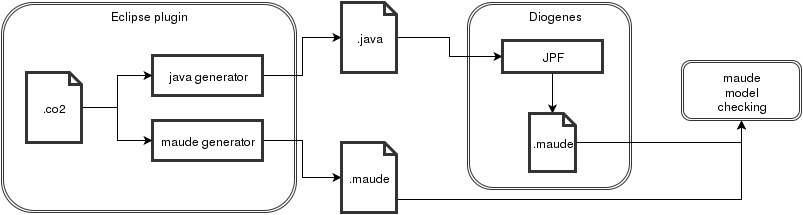
\includegraphics[width=\textwidth]{img/diogenes-arch.png}
    \caption{Data flow schema}
    \label{fig:data-flow}
\end{figure}